\documentclass{standalone}
\usepackage{tikz}

\begin{document}

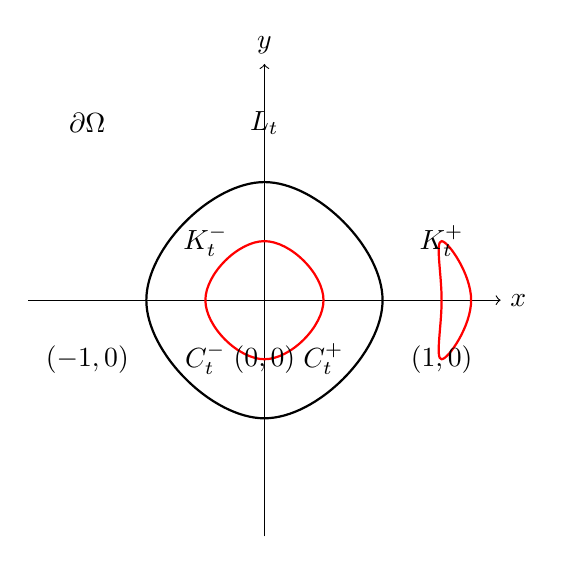
\begin{tikzpicture}[scale=1.5]
    % Draw the axes
    \draw[->] (-2,0) -- (2,0) node[right] {$x$};
    \draw[->] (0,-2) -- (0,2) node[above] {$y$};

    % Draw the curves
    \draw[thick] plot [smooth cycle,tension=0.8] coordinates {(-1,0) (0,1) (1,0) (0,-1)};
    \draw[red, thick] plot [smooth cycle,tension=0.8] coordinates {(-0.5,0) (0,0.5) (0.5,0) (0,-0.5)};
    \draw[red, thick] plot [smooth cycle,tension=0.8] coordinates {(1.5,0) (1.5,0.5) (1.75,0) (1.5,-0.5)};

    % Label the curves
    \node at (-0.5,0.5) {$K_t^-$};
    \node at (1.5,0.5) {$K_t^+$};
    \node at (0,1.5) {$L_t$};
    \node at (-1.5,1.5) {$\partial\Omega$};
    \node at (-1.5,-0.5) {$( -1, 0 )$};
    \node at (1.5,-0.5) {$( 1, 0 )$};
    \node at (0,-0.5) {$( 0, 0 )$};
    \node at (0.5,-0.5) {$C_t^+$};
    \node at (-0.5,-0.5) {$C_t^-$};
\end{tikzpicture}

\end{document}